\documentclass[a4paper,twoside,12pt]{report}
% Richard Klein (2020,2021)

% Include Packages
%\usepackage[a4paper,inner=3.5cm,outer=2.5cm,top=2.5cm,bottom=2.5cm]{geometry}  % Set page margins
\usepackage{fullpage}
\usepackage{float}                  % Allows 'Here and Only Here' [H] for Floats
\usepackage{url}                    % \url{} command
\usepackage{charter}                  % Set font to Times
\usepackage{graphicx}               % \includegraphics
\usepackage{subfigure}              % Allow subfigures
\usepackage{amsmath}
\usepackage{amssymb}
\usepackage{amsthm}
\usepackage{booktabs}
\usepackage{parskip}
\usepackage[all]{nowidow}
\setnoclub[2]
\setnowidow[2]

% Referencing
% Provides \Vref and \vref to indicate where a reference is.
\usepackage{varioref} 
% Hyperlinks references
\usepackage[bookmarks=true,bookmarksopen=true]{hyperref} 
% Provides \Cref, \cref, \Vref, \vref to include the type of reference: fig/eqn/tbl
\usepackage{cleveref} 
% Setup Hyperref
\hypersetup{
  colorlinks   = true,              %Colours links instead of ugly boxes
  urlcolor     = blue,              %Colour for external hyperlinks
  linkcolor    = blue,              %Colour of internal links
  citecolor    = blue                %Colour of citations
}
% Names for Clever Ref
\crefname{table}{table}{tables}
\Crefname{table}{Table}{Tables}
\crefname{figure}{figure}{figures}
\Crefname{figure}{Figure}{Figures}
\crefname{equation}{equation}{equations}
\Crefname{equation}{Equation}{Equations}

% Wits Citation Style
\usepackage{natbib} % Force natbib.sty to put citation labels in the reference list
\makeatletter
\renewcommand\NAT@biblabel[1]{\def\citeauthoryear##1##2{##1 ##2}[#1]\hfill}
\renewcommand\NAT@bibsetup[1]{%
  \setlength{\itemsep}{\bibsep}\setlength{\parsep}{\z@}}
\def\@lbibitem[#1]#2{%
  \if\relax\@extra@b@citeb\relax\else
    \@ifundefined{br@#2\@extra@b@citeb}{}{%
     \@namedef{br@#2}{\@nameuse{br@#2\@extra@b@citeb}}}\fi
   \@ifundefined{b@#2\@extra@b@citeb}{\def\NAT@num{}}{\NAT@parse{#2}}%
   \item[\hfil\hyper@natanchorstart{#2\@extra@b@citeb}\@biblabel{#1}%
    \hyper@natanchorend]%
    \NAT@ifcmd#1(@)(@)\@nil{#2}}
\makeatother


\bibliographystyle{named-wits}
\bibpunct{[}{]}{;}{a}{}{}  % to get correct punctuation for bibliography
\setlength{\skip\footins}{1.5cm}
\newcommand{\citets}[1]{\citeauthor{#1}'s \citeyearpar{#1}}
\renewcommand\bibname{References}  

\pagestyle{headings}

\pagestyle{plain}
\pagenumbering{roman}

\renewenvironment{abstract}{\ \vfill\begin{center}\textbf{Abstract}\end{center}\addcontentsline{toc}{section}{Abstract}}{\vfill\vfill\newpage}
\newenvironment{declaration}{\ \vfill\begin{center}\textbf{Declaration}\end{center}\addcontentsline{toc}{section}{Declaration}}{\vfill\vfill\newpage}
\newenvironment{acknowledgements}{\ \vfill\begin{center}\textbf{Acknowledgements}\end{center}\addcontentsline{toc}{section}{Acknowledgements}}{\vfill\vfill\newpage}

\begin{document}
\onecolumn
\thispagestyle{empty}

\setcounter{page}{0}

\begin{center}
  \vfill
  {
  \huge \bf \textsc{The Optimization of Wireless Communication in the AI\_r Air Quality Monitoring System used in Underground Mines}
  \vspace{50pt}\\
  \large School of Computer Science \& Applied Mathematics\\
  \large University of the Witwatersrand\\[20pt]
  \normalsize
  Alexandra Barry\\
  1056862\\[20pt]
  Supervised by Bruce Mellado\\[10pt]
  \today
  }

  \vfill
  \vfill
  
\includegraphics[width=1.5cm]{images/wits}
  \vspace{10pt}\\
  \small{A proposal submitted to the Faculty of Science, University of the Witwatersrand, Johannesburg,
in partial fulfilment of the requirements for the degree of Master of Science}\\
\end{center}
\vfill
\newpage

\pagestyle{plain}
\setcounter{page}{1}

\phantomsection
\begin{declaration}
I, Alexandra May Barry, hereby declare the contents of this research proposal to be my own work.
This proposal is submitted as a requirement for the course 'COMS7060' within of the degree of Master of Science in Robotics at the University of the Witwatersrand.
This work has not been submitted to any other university, or for any other degree.
\end{declaration}

\phantomsection
\begin{abstract}
Air quality monitoring is an important aspect of ensuring safe and healthy living and working environments. Readings and predictions of air quality can assist governing bodies in applying appropriate mitigation steps and policies to reduce air pollution where necessary. The South African Consortium of Air Quality Monitoring (SACAQM) developed a low cost monitoring system, 'AI\_r', that comprises of IoT sensor nodes connected to the cloud. The readings of these are processed with machine learning algorithms to provide accurate real-time predictions. 
\newline \newline
This report examines the practicality of extending the AI\_r system into a mining context and analyzes the methods that can be employed to optimize the wireless communication methods and power use of the system.
\end{abstract}

\phantomsection
\tableofcontents
\newpage
\phantomsection
\addcontentsline{toc}{section}{List of Figures}
\listoffigures
\newpage
\phantomsection
\addcontentsline{toc}{section}{List of Tables}
\listoftables
\newpage
\pagenumbering{arabic}

\chapter{Introduction}
[Introduction]

[brief on air quality]

[brief on AI\_r system developed]

[importance of extending to mining and gap in current research]

[explanation of sections]

\chapter{Background and Related Work}
[The literature review shows a familiarity with
the literature relevant to the project and motivates the research problem or question.
]
\section{Introduction}
This chapter details the existing project: 'AI\_r' for which this research is an extension of, examines the importance of air quality monitoring and explores related research and similar projects.

\section{Background}
\subsection{Air Quality Monitoring}

... Discuss air quality monitoring
This is just a paragraph

Many harmful aerosols, including: quarts, silica, arsenic, diesel and particulate matter are generated during the mining process and this affects miners both under and above ground\citep{Hercus_2022}. Real-time, accurate air quality measurements are critical to assist in monitoring whether exposure is above regulatory limits. These readings can be used to warn miners or can indicate the need for improved ventilation and mining operation mechanisms. It's estimated that 50\% of the energy consumed in mining operations is due to the ventilation systems\citep{Hercus_2022}. Integrating air quality measurements into an automated ventilation control system could provide a cost-effective method of ensuring a healthy supply of fresh air to the miners. 

\subsection{The SACAQM AI\_r System}
\subsubsection{Purpose}
The AI\_r system was developed as a solution to the high cost and complexity of traditional air quality monitoring stations\citep{SACAQM}. It will supplement the existing national quality monitoring systems by adding hundreds of thousands of additional sensor nodes. The system is comprised of air quality sensors within an IoT network, powered by Artificial Intelligence with the aim of providing accurate prediction and analysis of air quality in real time\citep{SACAQM}.

\subsubsection{Sensor Node Architecture}
Text

Nodes equipped with the following sensor suite: ambient temperature, relative humidity, ambient pressure, SO2, NO, NO2, PM2.5, PM10.

Master nodes: 
- high-quality measurement of PM2.5 and other measurements
- these require significant electrical power - battery powered
- connected to cloud via 4G networks
- designed to be self-sufficient for up to 1 year with battery power
- SEN55x sensor
- nRF5160 SiP

Slave nodes:
- less accurate PM2.5 sensors, used to create alerts of poor quality air conditions
- communicate with other master nodes through LoRa
- solar cell powered
- nRF52840 SoC
- 

\begin{figure}[ht]
	\centering
	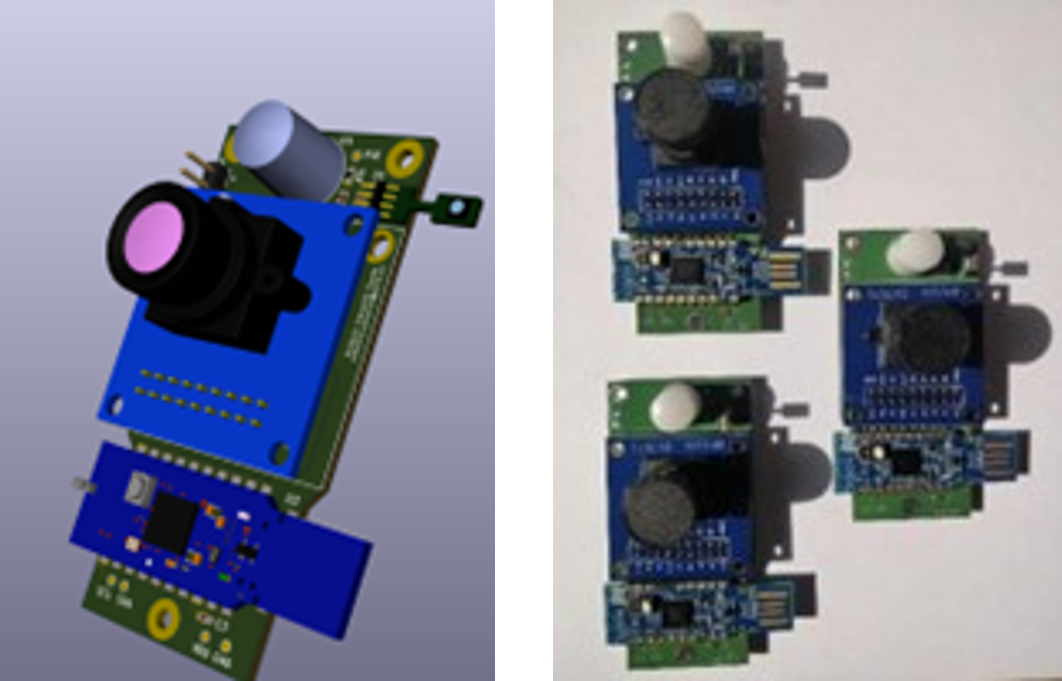
\includegraphics[width=0.6\linewidth]{images/SensorNodes.png}
	\caption{AI\_r Sensor Nodes}
	\label{fig:SensorNodes}
\end{figure}


\begin{figure}[ht]
	\centering
	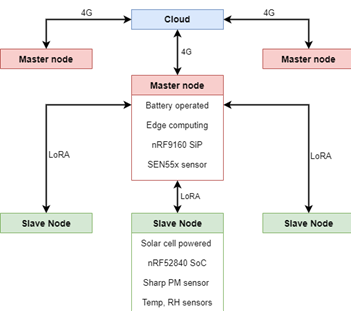
\includegraphics[width=0.5\linewidth]{images/Network_topology_of_AI_r_system_cropped.png}
	\caption{Network Topology of AI\_r System}
	\label{fig:NetworkTopology}
\end{figure}



\subsection{Wireless Communication}
[Wireless communication methods used in the system are...]
\subsubsection{LoRa}

\begin{figure}[ht]
	\centering
	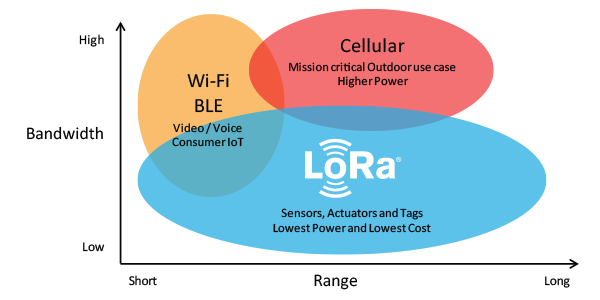
\includegraphics[width=0.5\linewidth]{images/LoRa_Why_Range.png}
	\caption{Diagram of LoRa Range, taken from \cite{Semtech_2023}}
	\label{fig:LoRaRange}
\end{figure}

Text \Cref{fig:LoRaTransmissionSpectogram}

\begin{figure}[ht]
	\centering
	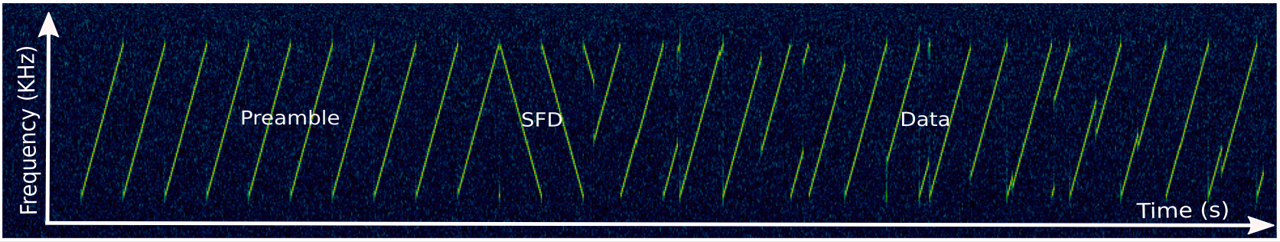
\includegraphics[width=0.8\linewidth]{images/LoRa transmission spectogram.png}
	\caption{Spectogram of LoRa Transmission, taken from \cite{Liando2019KnownStudy}}
	\label{fig:LoRaTransmissionSpectogram}
\end{figure}


\begin{enumerate}
    \item Network Topologies
    \item Performance Metrics
\end{enumerate}

\begin{figure}[ht]
	\centering
	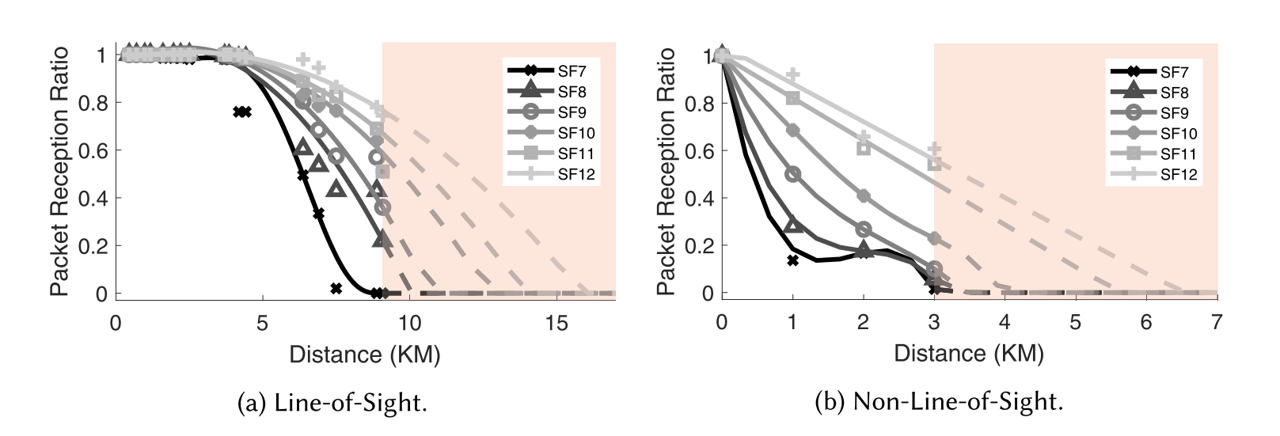
\includegraphics[width=0.8\linewidth]{images/LoRa_propagation_line_of_sight.png}
	\caption{Communication Distances for Varying Spreading Factors in Different Environments, taken from \cite{Liando2019KnownStudy}}
	\label{fig:LoRaTransmissionSpectogram}
\end{figure}

\^ communication is fine up to 9km for line-of-sight environments but propagation is impacted when obstructed


Figure captions are at the bottom. Table title are at the top of the table as seen in \Vref{tab:tab1}. There is a package called BookTabs which is \textit{way} better for tables and you should learn how to use that instead.

\begin{table}[p]
	\centering
	\caption{LoRa Chipset Configuration Options as Described in \cite{SemtechDatasheet}}
	\label{tab:tab1}
\begin{tabular}{cc}
	\hline
	Parameter & Options\\
	\hline\hline 
	SF & 6, 7, 8, 9, 10, 11, 12 \\ 
	BW (kHz) & 7.8, 10.4, 15.6, 20.8, 31.2, 41.7, 62.5, 125, 250, 500 \\ 
    CR & 4/5, 4/6, 4/7, 4/8 \\ 
    IH & True or False \\ 
    DE & True of False (recommended True for $T_{sym} > 16ms$) \\ 
    IH & True (uplink) or False (downlink) \\ 
    IH & 0-255 Bytes \\ 
    IH & 6-65,535 symbols \\ 
	\hline
\end{tabular} 
\end{table}

Recommendation: SF settings SF7 to SF12 and BW 125, 250 and 500kHz \cite{SemtechDatasheet}

\subsection{Mining Environment}
\subsubsection{Typical Mining Architectures}
\subsubsection{Network Interference in Mining Context}

\section{Related Work}

\subsubsection{Analyses of LoRa Networks}
Performance Determinants in LoRa Networks: A Literature Review \cite{Gkotsiopoulos2021PerformanceReview}

Known and Unknown Facts of LoRa Experiences from a Large scale Measurement Study \cite{Liando2019KnownStudy}

\subsubsection{IoT Systems in Underground Contexts}

An Internet of Things System for Underground Mine Air Quality Pollutant Prediction Based on Azure Machine Learning \cite{Jo_Khan_2018} -- Arduino, ZigBee

Monitoring System for Coal Mine Safety Based on Wireless Sensor Network \cite{Zhu2019MonitoringNetwork} -- zigbee

Improving coal mine safety with internet of things (IoT) based Dynamic Sensor Information Control System \cite{Ali2022ImprovingSystem} 

Applications of wireless sensor networks to improve occupational and health in underground mines \cite{Sadeghi2022ApplicationsMines}

DeepSense: Sensing the Radio Signal Behavior in Metal and Non-Metal Underground Mine Workings \cite{Ranjan2018DeepSense:Workings}

\chapter{Research and Methodology}
[The candidate shows a familiarity with the
methods available for solving the research
problem or answering the research question,
and the chosen methods are well-motivated.]

\section{Introduction and Problem Statement}
air quality importance
use in mining space to prevent disease
need for effective IoT systems
existing AI\_r system
extension of that includes networks that may not be suited to mining context
need to analyze how these can be optimized for power and SNR

\section{Research Question}
[The research problem or question is clear, sufficiently narrow, and solvable or answerable
within the constraints of the project.]
\newline


- Are there adjustments to the networks used that would need to be made for a mining environment
- How can the parameters and features of the selected networks be optimized for performance in a mining context
- Are the selected networks in the system sufficient for coping in a mining environment
\section{Research Aims and Objectives}

- reduction of data by analyzing sensors required for predictions
- selection of radio parameters for optimized communication in mining environment
- 

\subsection{Research Aims}
[The aim and objectives are relevantly related
to the research problem or question.]
\newline
The aims of the research include:
\begin{itemize}
    \item Determining whether the existing features of the AI\_r system are suitable to be used in a mining context or whether modifications to the architecture would need to be made
    \item Determining what set of parameters can be adjusted to optimize the collection of sensor data in terms of power usage and transmission reliability
\end{itemize}

\subsection{Objectives}
The objectives of the research include:
\begin{itemize}
    \item Determining whether the existing features of the AI\_r system are suitable to be used in a mining context or whether modifications to the architecture would need to be made
    \item Determining what set of parameters can be adjusted to optimize the collection of sensor data in terms of power usage and transmission reliability
\end{itemize}

\section{Research design}
\section{Methods}
- Analysis of research in various networks and performance within mining context
- Development of a test scenario in the Wits mock mine shaft
- Assess effects of varying LoRa parameters (SF, BW, Tx Power)
- Optimization in terms of power - solar cells will not be feasible in mining context
- SNR performance and battery most important

RFM95W LoRa radio with Arduino readings taken on PC of RSSI and SNR

The nodes were tested with every viable bandwidth and spreading factor i.e. 125kHz & 250kHz with SF7-12
They were tested for received power RSSI and the SNR of the received signal
All tests were performed at maximum transmit power (20dBm) as distance can be roughly extrapolated from there and ultimately the power consumption is not high.


\section{Limitations}

Testing considerations
While the metal infrastructure may cause some sort of interference the testing is not indicative of a real shaft as we cannot measure the effect of reflections of the rough mine surface as well as any tilt effects of the tunnel
Exact dimensions in terms of height unknown so unable to make any distance related extrapolations
Since Shafts are usually somewhat straight and directional, setting up Line of Sight for the nodes is realistic.

\chapter{Schedule of Work}
[The schedule of work is sufficiently detailed
and is feasible
]
\section{Schedule of Work}
Phases:


\begin{table}[p]
	\centering
	\caption{Proposed Schedule of Work for Capstone Project}
	\label{tab:workScheduleTable}
\begin{tabular}{ccc}
	\hline
	Week & Activity & Hours\\
	\hline\hline 
	July 17 & activity & 0 \\ 
	24 & activity & 0 \\ 
    31 & activity & 0 \\ 
    \hline
    Aug 7 & activity & 0 \\ 
    14 & activity & 0 \\ 
    21 & activity & 0 \\ 
    28 & Report write-up & 20 \\ 
    \hline
    Sep 4 & \textit{Mid-term Vacation} & - \\ 
    11 & Final changes to report & 6 \\ 
    \textbf{12} & \textbf{Capstone Project Report Due} & - \\ 
    18 & Preparation for presentation & 10 \\
    25 & Presentation preparation and creation of project poster & 20 \\
    \textbf{27} & \textbf{Capstone Project Presentation} & - \\ 
	\hline
    Oct 2 & Creation and finalization of project poster & 10 \\
    \textbf{6} & \textbf{Capstone Project Poster Due} & - \\ 
    \hline
\end{tabular} 
\end{table}

\nocite{*}

\bibliography{references, references-mendeley}\addcontentsline{toc}{chapter}{References}
\end{document}
